\section{Inpainting}
\label{sec:Inpainting}
\subsection{Bakgrunn}
Inpainting er en utbredt teknikk innenfor bildebehandling \cite{wiki:inpainting}. Teknikken kan brukes til å fylle inn manglende informasjon eller fjerne uønsket støy eller elementer i bilder \footnote{Poisson Image Editing\cite{papers0171:online}}. Selvom kunsten å reparere gamle og forfalne bilder har eksistert i mange år, har det nylig opplevd en økning i popularitet grunnet den raske utviklingen av bildebehandlingsteknikker. Bilder er for tiden en av de mest vanlige formene for informasjon. Derfor er teknikker som kan endre bilder uten spor blitt et sikkerhetsproblem. Et eksempel på dette er den svært utbredte delingen av personlige bilder i sosiale medier. Disse kan inneholde objekter som lett kan fjernes for å drastisk endre semantikken i hele bildet. Fjerning av visse elementer er i tillegg sett på som en løsning for forfalskning av bilder. Litteraturen som beskriver fjerning av objekter deles gjerne inn i to kategorier: inpainting og kloning. Kloning blir diskutert i detalj i (\ref{sec:kloning}). Tidligere ble inpainting i større grad brukt på gamle bilder for å fjerne riper o.l. I nyere tid brukes det mer for å fjerne gjenstander som har blitt lagt til i bilder. I tillegg brukes inpainting til å fjerne forstyrrelser som linjer, flekker og tekst \cite{1909063938:online}.

\subsection{Teori}
 Metoden går ut på å fylle informasjon i et ønsket området ut fra informasjon i det omkringliggende området. Dette gjøres ved å sette $h=0$ i $\Omega_i$ og løse likning~(\ref{eq:eksplisitt}) i $\Omega_i$, dersom $\Omega_i \subset \Omega$ er det området hvor inpaintingen skal utføres. Implementasjonen i dette prosjektet krever at en fornuftig maske velges for at resultatet skal oppleves tilfredsstillende. NVIDIA har implementert en algoritme som bruker deep learning \cite{wiki:Deep_learning}, hvor tilsynelatende ødelagte bilder kan gjenopprettes til meget høy kvalitet \cite{180407722:nvidia}, illustrert ved Figur \ref{fig:nvidia}. I vår implementasjon er man i større grad avhengig av at masken befinner seg på et gunstig sted slik at ikke viktig informasjon tildekkes.
 
 \subsection{Implementasjon}
 For implementasjon i Python konstrueres en maske i form av en bool-array som er sann for alle piksler innenfor målområdet $\Omega_i$, og usann utenfor.

\begin{lstlisting}[language=Python]
mask = np.zeros(im.shape)    #lag maske
mask[135:140, 250:380] = 1
mask[250:470, 300:305] = 1
mask[740:755, 550:700] = 1
mask = mask.astype(bool)    #lag bool-array
\end{lstlisting}
 
Deretter bruker man denne arrayen som en "view" \footnote{\url{https://docs.scipy.org/doc/numpy/user/basics.indexing.html}} på array-representasjonen av bildet for å løse diffusjonslikningen~(\ref{eq:eksplisitt}) innenfor området $\Omega_i$, før man sender med array-representasjonen og masken til funksjonen som løser diffusjonslikningen eksplisitt med dirichlet randbetingelser. For hver iterering blir området innenfor målområdet satt til å være likt tilsvarende område i originalbildet.
\begin{lstlisting}[language=Python]
    im[~mask] = im0[~mask]
\end{lstlisting}
Tilslutt returneres originalbildet og det ferdig inpaintede bildet fra funksjonen som løste diffusjonslikningene. Figur \ref{fig:inpaint} viser resultatet av vår inpaintingalgoritme, her med \texttt{n=100} iterasjoner. Her ble masken definert som 3 rette svarte klosser. Etter inpainting er fullført er de tilsynelatende borte. 
\begin{figure}
\begin{center}
    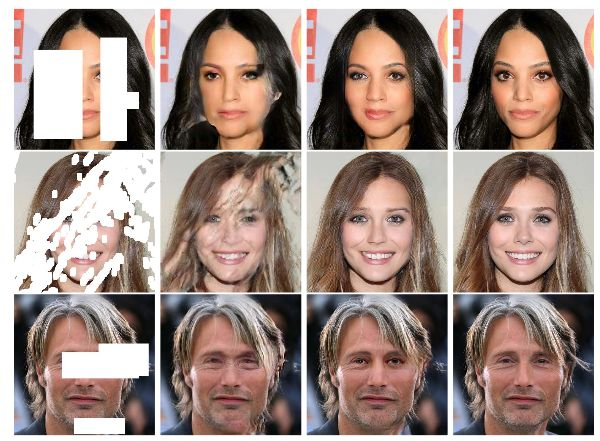
\includegraphics[width=0.6\columnwidth]{bilder/nvidia-image-inpainting-demo.jpg}
    \caption{NVIDIAs inpaintingalgoritme~ \label{fig:nvidia}}
    \source{NVIDIA~\cite{NVIDIADe38:online}}
\end{center}
\end{figure}

\begin{figure}
\begin{center}
    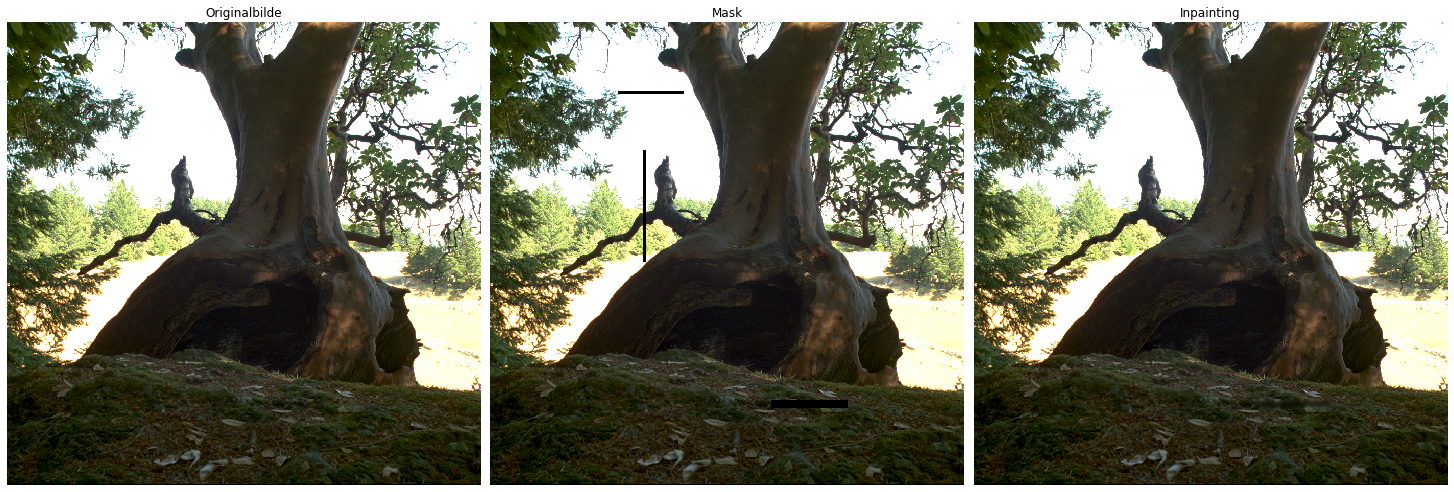
\includegraphics[width=1\columnwidth]{bilder/tree_inpaint.png}
    \caption{Inpainting av tre~ \label{fig:inpaint}}
\end{center}
\end{figure}
